
%%%%%%%%%%%%%%%%%%%%%%% file typeinst.tex %%%%%%%%%%%%%%%%%%%%%%%%%
%
% This is the LaTeX source for the instructions to authors using
% the LaTeX document class 'llncs.cls' for contributions to
% the Lecture Notes in Computer Sciences series.
% http://www.springer.com/lncs       Springer Heidelberg 2006/05/04
%
% It may be used as a template for your own input - copy it
% to a new file with a new name and use it as the basis
% for your article.
%
% NB: the document class 'llncs' has its own and detailed documentation, see
% ftp://ftp.springer.de/data/pubftp/pub/tex/latex/llncs/latex2e/llncsdoc.pdf
%
%%%%%%%%%%%%%%%%%%%%%%%%%%%%%%%%%%%%%%%%%%%%%%%%%%%%%%%%%%%%%%%%%%%

\UseRawInputEncoding
\documentclass[a4paper]{llncs}

\usepackage{amssymb}
\setcounter{tocdepth}{3}
\usepackage{graphicx}
\usepackage{listings}
\usepackage{xcolor}
\usepackage[utf8]{inputenc}
\usepackage[T1]{fontenc}

\lstset{
  basicstyle=\ttfamily\footnotesize,
  keywordstyle=\color{blue},
  commentstyle=\color{gray},
  stringstyle=\color{orange},
  showstringspaces=false,
  breaklines=true,
  frame=single,
  captionpos=b
}


\usepackage{url}
\urldef{\mailsa}\path|flchayle@outlook.com, antonela.tommasel@isistan.unicen.edu.ar|
\newcommand{\keywords}[1]{\par\addvspace\baselineskip
\noindent\keywordname\enspace\ignorespaces#1}

\begin{document}

\mainmatter  % start of an individual contribution

% first the title is needed
\title{Una Arquitectura Híbrida Extensible para Sistemas IA-Ready}

% a short form should be given in case it is too long for the running head
\titlerunning{Una Arquitectura Híbrida Extensible para Sistemas IA-Ready}

% the name(s) of the author(s) follow(s) next
%
% NB: Chinese authors should write their first names(s) in front of
% their surnames. This ensures that the names appear correctly in
% the running heads and the author index.
%
\author{Facundo Leonardo Chayle\inst{1} \and Antonela Tommasel\inst{2}}

%
\authorrunning{Una Arquitectura Híbrida Extensible para Sistemas IA-Ready}
% (feature abused for this document to repeat the title also on left hand pages)

% the affiliations are given next; don't give your e-mail address
% unless you accept that it will be published
\institute{
\inst{1} Universidad Abierta Interamericana. Facultad de Tecnología Informática.\\
Centro de Altos Estudios en Tecnología Informática. Buenos Aires. Argentina
\and
\inst{2} Universidad Nacional del Centro de la Provincia de Buenos Aires (UNICEN).\\
ISISTAN-CONICET. Tandil. Argentina\\
\mailsa
}

%
% NB: a more complex sample for affiliations and the mapping to the
% corresponding authors can be found in the file "llncs.dem"
% (search for the string "\mainmatter" where a contribution starts).
% "llncs.dem" accompanies the document class "llncs.cls".
%

\toctitle{Lecture Notes in Computer Science}
\tocauthor{Authors' Instructions}
\maketitle


\begin{abstract}
La creciente integración de inteligencia artificial en sistemas de software exige arquitecturas mucho más flexibles, escalables y adaptables al contexto. Este trabajo propone una arquitectura híbrida extensible que combina principios de microservicios, ejecución paralela y edge computing, permitiendo una incorporación efectiva de capacidades de IA en distintos dominios. La solución se complementa con mecanismos innovadores como orquestación dinámica, seguridad Zero Trust AI y aprendizaje autónomo, orientados a resolver limitaciones presentes en enfoques tradicionales. Para validar su aplicabilidad, se presenta un scaffolding funcional implementado en FastAPI y NestJS, demostrando su carácter modular y agnóstico al lenguaje. Esta propuesta busca facilitar el diseño de sistemas IA-ready robustos, seguros y sostenibles, ofreciendo una alternativa viable para entornos complejos y heterogéneos.
\keywords{Arquitectura híbrida extensible, Inteligencia artificial, Microservicios, Edge computing, Zero Trust AI, Aprendizaje autónomo}
\end{abstract}


\section{Introducción y Motivación}

La creciente integración de capacidades de inteligencia artificial (IA) en sistemas de software modernos ha dado lugar a un cambio de paradigma en el diseño de arquitecturas tecnológicas. Desde sistemas de recomendación hasta asistentes conversacionales, pasando por modelos generativos y clasificadores en tiempo real, los componentes de IA se han convertido en piezas centrales de muchas
soluciones digitales actuales. Sin embargo, su adopción masiva también ha evidenciado desafíos estructurales relevantes: falta de modularidad, dificultades de escalabilidad, rigidez ante contextos dinámicos, problemas de gobernanza sobre los modelos desplegados y limitaciones en la interoperabilidad entre componentes inteligentes y lógicos~\cite{amershi2019software,schlegel2022artifact}.

Para comprender en profundidad estas limitaciones, se llevó a cabo un Mapeo Sistemático de la Literatura~\cite{chayle2024msl}, el cual permitió analizar más de 80 trabajos científicos publicados en los últimos cinco años. A partir de este análisis, se identificó una escasa presencia de soluciones arquitectónicas que contemplen de forma integral aspectos como: separación entre lógica de negocio e inteligencia artificial, soporte para ejecución en entornos distribuidos (incluido \emph{edge computing}), y mecanismos de gobernanza adaptativa. La mayoría de las propuestas se enfocaban en soluciones verticales y altamente acopladas a dominios específicos, sin ofrecer lineamientos reutilizables o adaptables para contextos diversos.

Frente a este panorama, surge la necesidad de diseñar una arquitectura genérica, adaptable y modular que permita integrar IA de forma escalable, segura y mantenible. Se requiere una propuesta que supere los enfoques tradicionales, permitiendo una separación de preocupaciones entre los modelos inteligentes y los servicios de negocio, y que al mismo tiempo facilite su ejecución tanto en la nube como en entornos periféricos.

Este trabajo propone una arquitectura híbrida extensible, que combina principios de microservicios, ejecución paralela y \emph{edge computing}. La propuesta incorpora mecanismos innovadores de orquestación dinámica, aprendizaje autónomo y seguridad mediante \emph{Zero Trust AI}. Para validar la viabilidad técnica del enfoque, se desarrolló un \emph{scaffolding} funcional implementado en dos tecnologías (FastAPI y NestJS), demostrando su carácter agnóstico al lenguaje y su aplicabilidad en contextos reales.

\subsection*{Objetivos}

Los objetivos de este trabajo son los siguientes:

\begin{itemize}
    \item Diseñar una arquitectura extensible para la integración de IA en sistemas de software, con foco en modularidad, adaptabilidad y gobernabilidad.
    \item Incorporar mecanismos de orquestación dinámica, seguridad proactiva y aprendizaje autónomo como innovaciones diferenciales.
    \item Validar la propuesta mediante un \emph{scaffolding} funcional implementado en dos tecnologías distintas (FastAPI y NestJS).
    \item Contribuir al debate académico y técnico sobre arquitecturas IA-ready, ofreciendo una base sólida para futuras investigaciones y desarrollos.
\end{itemize}



\section{Estado del Arte}

La integración de inteligencia artificial (IA) en arquitecturas de software ha evolucionado aceleradamente, impulsada por la necesidad de escalar soluciones inteligentes en sectores como la salud, manufactura, educación y servicios digitales. Los enfoques predominantes han girado en torno a arquitecturas de microservicios, \textit{pipelines} secuenciales de inferencia, y despliegues \textit{serverless}, en un intento por mejorar la mantenibilidad, escalabilidad y flexibilidad de los sistemas.

Kumar et al.~\cite{kumar2024serverlessai} examinan la combinación de arquitecturas \textit{serverless} con modelos de aprendizaje automático como una estrategia emergente para despliegue escalable con baja complejidad operativa. Aunque identifican ventajas como el autoescalado y la reducción de costos, también destacan desafíos como la latencia de \textit{cold start} y la falta de estado persistente en las funciones. Por su parte, Song et al.~\cite{song2023surveyserverless} realizan un relevamiento exhaustivo sobre la inferencia de modelos en entornos \textit{serverless}, discutiendo limitaciones asociadas al rendimiento, uso de GPU y tiempos de respuesta.

En relación con MLOps, el trabajo de Nguyen-Duy et al.~\cite{nguyenduy2022mlops} presenta una visión general de la operación de modelos de aprendizaje automático, abordando aspectos como automatización del ciclo de vida, monitoreo y gobernanza. No obstante, estos enfoques suelen estar acotados a la nube y no consideran ejecución en el borde ni mecanismos de orquestación adaptativa en función del contexto.

A pesar de estos avances, persisten vacíos críticos que limitan la aplicabilidad general de estas arquitecturas:

\begin{itemize}
  \item \textbf{Modularidad e independencia del dominio:} la mayoría de las soluciones siguen siendo específicas de dominio, sin ofrecer lineamientos reutilizables~\cite{arora2022modular}.
  \item \textbf{Ejecución híbrida \textit{cloud-edge}:} el \textit{edge computing} ha sido explorado en contextos aislados, pero sin mecanismos estandarizados para su integración con la nube~\cite{satyanarayanan2017emergence}.
  \item \textbf{Orquestación dinámica de modelos IA:} son escasas las propuestas que implementan selección adaptativa de modelos según contexto o carga del sistema~\cite{deng2024orchestrated}.
  \item \textbf{Seguridad centrada en IA:} no se evidencian marcos de control de datos específicos para flujos inteligentes ni validaciones contextuales~\cite{yang2023zerotrust}.
  \item \textbf{Aprendizaje autónomo y autosustentable:} pocas arquitecturas contemplan mecanismos de reentrenamiento o adaptación automática a nuevos datos.
\end{itemize}

Un Mapeo Sistemático de la Literatura (MSL) reciente~\cite{chayle2024msl}, que analizó más de 80 trabajos publicados entre 2018 y 2024, confirmó la escasez de propuestas que integren estos aspectos de forma holística. En consecuencia, resulta necesaria una arquitectura genérica, adaptable y extensible que permita integrar IA en distintos contextos sin comprometer la gobernabilidad, la seguridad ni la escalabilidad del sistema.






\section{Propuesta Arquitectónica}

Este trabajo propone una \textbf{arquitectura híbrida extensible} para la integración de capacidades de inteligencia artificial en sistemas de software. La propuesta se apoya en tres pilares fundamentales: separación de responsabilidades entre IA y lógica de negocio, soporte para ejecución híbrida (cloud y edge), y modularidad para facilitar su adaptación a distintos dominios. 

La arquitectura está compuesta por los siguientes bloques principales:

\begin{itemize}
    \item \textbf{Orchestration Service}: servicio principal que centraliza la lógica de negocio y la coordinación general del sistema. Implementado en NestJS, este componente expone los endpoints del dominio, invoca al servicio de IA cuando es necesario, y contiene un orquestador dinámico capaz de seleccionar modelos según el contexto.
    
    \item \textbf{AI Service}: microservicio especializado en procesamiento inteligente, implementado en FastAPI. Contiene la lógica de inferencia, validación de entradas, preprocesamiento y postprocesamiento. Es independiente del dominio y fácilmente intercambiable o escalable.
    
    \item \textbf{Edge Agent (opcional)}: componente ligero que permite ejecutar inferencias localmente en entornos con restricciones de conectividad o latencia. Es configurable y puede adaptarse a diferentes escenarios de borde.
    
    \item \textbf{Canal de comunicación}: el sistema puede operar tanto mediante HTTP REST como a través de eventos asincrónicos (por ejemplo, usando WebSockets o colas de mensajes), permitiendo flexibilidad en la forma de interacción.
\end{itemize}

A nivel de arquitectura, la lógica del orquestador permite seleccionar el motor de inferencia más adecuado en función del contexto operativo. Este mecanismo considera factores como la latencia, la disponibilidad del entorno edge y la carga del sistema para decidir dinámicamente si delegar la inferencia localmente o a través del servicio de IA remoto.

La Figura~\ref{fig:arquitectura} muestra una vista esquemática de esta propuesta.

\begin{figure}[h]
    \centering
    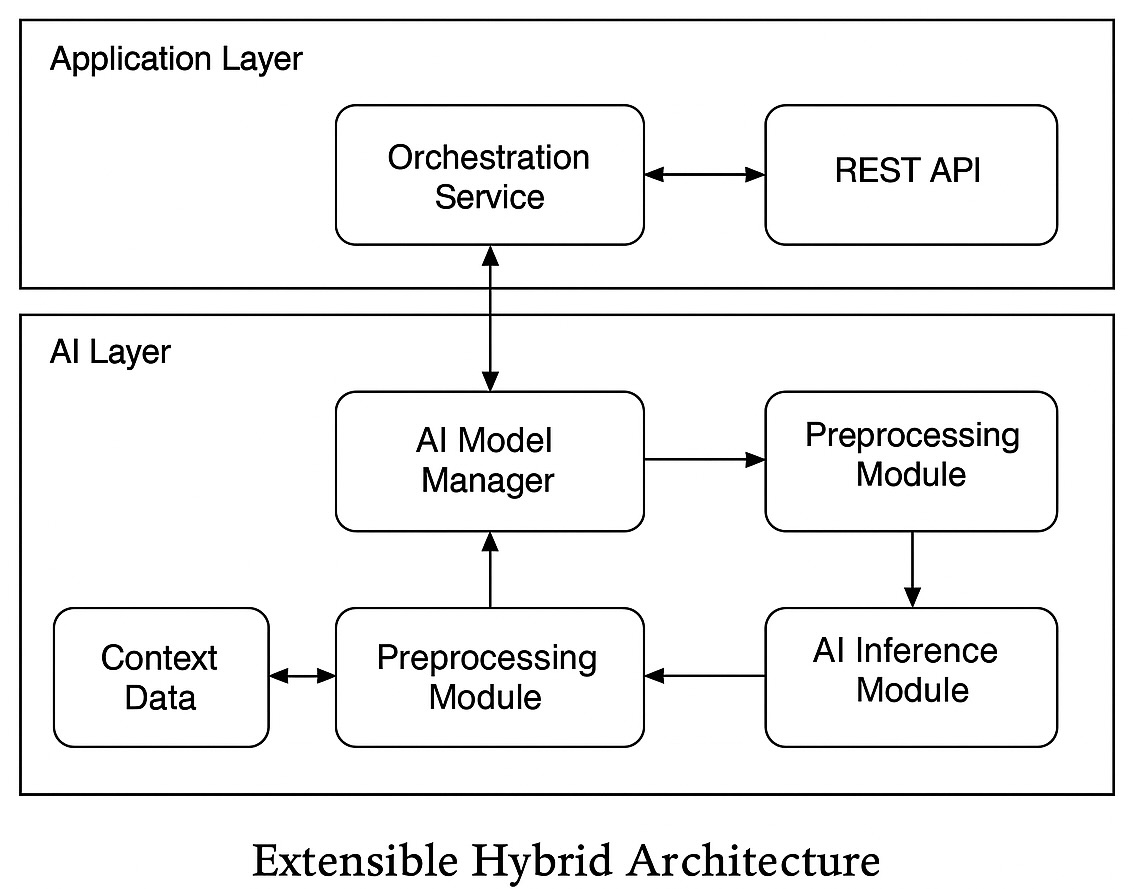
\includegraphics[width=0.8\linewidth]{A_flowchart_in_black_and_white_illustrates_the_ext.jpeg}
    \caption{Arquitectura híbrida extensible propuesta.}
    \label{fig:arquitectura}
\end{figure}

Este enfoque permite una incorporación progresiva de capacidades de IA sin comprometer la mantenibilidad del sistema base. Además, sienta las bases para futuras extensiones como selección dinámica de modelos, aprendizaje continuo y validación basada en principios Zero Trust AI.








\section{Scaffolding y Diseño de Implementación}

Con el objetivo de validar la viabilidad técnica de la propuesta, se desarrolló un \textit{scaffolding} funcional compuesto por dos servicios independientes: un microservicio de inferencia en FastAPI (Python) y un servicio de orquestación en NestJS. Esta elección tecnológica busca demostrar la independencia del enfoque y su aplicabilidad en entornos heterogéneos.

El microservicio de IA se organiza en capas claras: lógica de predicción, pre/post-procesamiento, esquemas de E/S y endpoints REST. El servicio de orquestación, por su parte, gestiona solicitudes del dominio, integra lógica de negocio, un cliente HTTP para invocar el microservicio de IA y un módulo de orquestación dinámica que selecciona modelos según el contexto. También incorpora eventos asíncronos, facilitando extensiones hacia arquitecturas reactivas.

Ambos servicios se comunican actualmente vía HTTP, aunque el diseño permite adoptar patrones asíncronos (eventos o colas) sin modificar la estructura base, reforzando así la flexibilidad del sistema.

\subsection*{Estructura del proyecto}


\begin{lstlisting}[basicstyle=\ttfamily, frame=single, caption={Estructura general del proyecto}]
project_root/
|- ai_service/               # Servicio de IA (FastAPI)
|  |- app/
|  |  |- main.py             # Punto de entrada FastAPI
|  |  |- inference/          # Logica de inferencia
|  |  |- api/                # Rutas REST
|  |  |- schemas/            # Validacion de datos
|  |  |- utils/              # Pre y post procesamiento
|  |- requirements.txt       # Dependencias Python
|- orchestration_service/    # Orquestacion (NestJS)
|  |- src/
|     |- main.ts             # Entrada NestJS
|     |- app.module.ts       # Modulo raiz
|     |- controllers/        # Endpoints del dominio
|     |- services/           # Logica de negocio
|     |- ai-client/          # HTTPClient hacia FastAPI
|     |- events/             # Gestion de Asincronismo
|     |- config/             # Configuracion
|  |- package.json           # Dependencias
|- edge_agent/               # Edge Agent (Opt.)
|  |- agent.py               # Inferencias Locales
|  |- config.json            # Configuracion
|- docker-compose.yml        # Docker
|- README.md                 # Descripcion general
\end{lstlisting}

\subsection*{Pseudocódigo de la interacción}

A continuación, se presenta un fragmento de pseudocódigo que describe la lógica simplificada del orquestador dinámico:

\begin{lstlisting}[language=Python, caption={Seleccion de motor IA segun contexto}]
def seleccionar_motor_ia(entrada, contexto):
    if contexto["latencia"] < 100 and contexto["edge_disponible"]:
        return EdgeAgent.inferir(entrada)
    else:
        return AIService.remoto_inferir(entrada)

def manejar_solicitud(dato_usuario):
    contexto = obtener_contexto()
    resultado = seleccionar_motor_ia(dato_usuario, contexto)
    return aplicar_reglas_de_negocio(resultado)
\end{lstlisting}

El proyecto esta estructurado para facilitar la adopción progresiva de la arquitectura en sistemas existentes. Cada componente puede evolucionar de forma independiente, permitiendo extender funcionalidades o reemplazar modulos sin afectar al resto del sistema. Esta modularidad tambien facilita la experimentación y evaluación comparativa de distintos modelos IA o estrategias de orquestación.







\section{Discusión y Comparación}

En esta sección se analizan las decisiones de diseño adoptadas y se comparan con enfoques existentes, destacando fortalezas, debilidades y aportes diferenciadores de nuestra propuesta.

\subsection{Comparación con arquitecturas existentes}

Las arquitecturas tradicionales basadas en microservicios, \textit{serverless} y \textit{pipelines} de IA han ofrecido soluciones modulares y escalables, pero presentan limitaciones claras:

\begin{itemize}
    \item Las propuestas de MLOps en la nube, como la de Nguyen-Duy et al.~\cite{nguyenduy2022mlops}, automatizan el ciclo de vida de los modelos, pero no contemplan procesamiento distribuido \textit{cloud-edge} ni orquestación basada en contexto.
    
    \item Soluciones \textit{serverless}, como las de Kumar et al.~\cite{kumar2024serverlessai} y Song et al.~\cite{song2023surveyserverless}, priorizan la elasticidad de recursos, pero presentan escasa interoperabilidad con la lógica de negocio.
    
    \item Propuestas híbridas \textit{cloud-edge}, como las de Liu et al.~\cite{liu2022edgecloud} y Morabito~\cite{morabito2018foggy}, introducen ejecución local, pero sin patrones estandarizados de orquestación dinámica ni capacidades de aprendizaje continuo.
\end{itemize}

Nuestra arquitectura propone una evolución de estos enfoques, integrando:

\begin{itemize}
    \item Microservicios desacoplados para modularidad y mantenibilidad.
    \item Ejecución híbrida con orquestación contextual basada en latencia, disponibilidad o privacidad.
    \item Validación proactiva con principios de \textit{Zero Trust AI}.
    \item Capacidades de autoaprendizaje y reentrenamiento autónomo.
\end{itemize}

\subsection{Innovaciones en el diseño}

Dos aspectos clave distinguen nuestra propuesta:

\textbf{Orquestación dinámica:} a diferencia de muchas arquitecturas tradicionales, esta propuesta incorpora un módulo central (en NestJS) que adapta dinámicamente la selección del modelo de IA en función del contexto operativo. Este enfoque se alinea con trabajos como Karimi \textit{et al.} (2023), que introducen patrones de orquestación por BPMN para microservicios IA~\cite{karimi2023dynamic}, y Deng \textit{et al.} (2024), quienes proponen workflows orquestados eficientes en arquitecturas distribuidas con ejecución dinámica~\cite{deng2024orchestrated}.

\textbf{Seguridad Zero Trust AI y autoaprendizaje:} mientras que gran parte de las arquitecturas existentes no contempla validación específica en flujos IA, nuestra solución implementa controles rigurosos de entrada/salida y pipelines para reentrenamiento autónomo basado en desempeño. Esto se encuentra en línea con estudios en privacidad-preservada y gobernanza de datos IA, como el de Huang \textit{et al.} (2022)~\cite{huang2022privacy}.

\subsection{Reflexión sobre decisiones de diseño}

\begin{itemize}
  \item \textbf{Elección tecnológica:} FastAPI y NestJS permiten demostrar independencia de lenguajes y facilitar adopción en entornos heterogéneos.
  \item \textbf{Separación de responsabilidades:} la separación entre servicios de IA y de negocio mejora escalabilidad y mantenibilidad.
  \item \textbf{Agente opcional en \textit{edge}:} permite ejecución local sin comprometer el diseño general.
  \item \textbf{Escalabilidad futura:} la arquitectura puede expandirse con tecnologías como Kubernetes, colas de eventos (Kafka, RabbitMQ) y monitoreo (Prometheus).
\end{itemize}

\subsection{Adopción en contextos regionales}

En entornos regionales, especialmente en América Latina, aún persisten barreras significativas para la adopción de arquitecturas modernas centradas en IA. Estas incluyen brechas en infraestructura digital, recursos limitados para la experimentación, falta de lineamientos técnicos claros y escasa transferencia desde el ámbito académico al productivo~\cite{campos2023artificial}. En ese sentido, el diseño modular y el \emph{scaffolding} replicable que proponemos pueden servir como punto de partida accesible para equipos de desarrollo locales que deseen implementar soluciones \emph{IA-ready} sin depender de plataformas complejas o costosas.

Este aspecto cobra especial relevancia considerando que la apropiación tecnológica en contextos con recursos limitados requiere enfoques escalables, desacoplados y comprensibles, principios que la presente arquitectura busca reflejar.

\subsection{Conclusión comparativa}

Nuestra arquitectura supera las limitaciones identificadas en el estado del arte al ofrecer una solución integral, flexible y escalable, con capacidad para operar en entornos heterogéneos e incorporar múltiples mecanismos de gobernanza, seguridad y adaptabilidad.





\section{Conclusiones}

La creciente complejidad de los sistemas que integran inteligencia artificial ha puesto de manifiesto la necesidad de arquitecturas más flexibles, escalables y adaptables al contexto. En este trabajo se ha propuesto una \textbf{arquitectura híbrida extensible} que busca responder a dichas exigencias mediante una combinación de microservicios, ejecución paralela, procesamiento en el borde y mecanismos avanzados de gobernanza de modelos.

A diferencia de muchas soluciones analizadas en la literatura, esta propuesta introduce componentes innovadores como un \textit{orquestador dinámico}, capaz de seleccionar en tiempo de ejecución el modelo de IA más adecuado, y mecanismos de \textit{seguridad Zero Trust AI}, que garantizan un flujo de datos validado y controlado de extremo a extremo. Asimismo, se incorpora la capacidad de \textit{autoaprendizaje y reentrenamiento autónomo}, permitiendo una adaptación continua ante cambios en los datos o el contexto operativo.

La implementación de un scaffolding funcional, basado en tecnologías ampliamente adoptadas como FastAPI y NestJS, demuestra la viabilidad técnica del enfoque y su carácter agnóstico al lenguaje. Este scaffolding no solo refleja los principios arquitectónicos propuestos, sino que también proporciona una base replicable para futuros desarrollos y adaptaciones.

Desde una perspectiva comparativa, la arquitectura desarrollada logra abordar de forma integral muchas de las limitaciones señaladas en el estado del arte, consolidando una propuesta robusta para el diseño de sistemas \textit{IA-ready}. En este sentido, el trabajo no solo ofrece una contribución conceptual, sino también una herramienta práctica para equipos de desarrollo, investigadores y arquitectos de software que buscan incorporar inteligencia artificial de forma controlada, escalable y gobernable.




\section{Trabajos Futuros}

Si bien la arquitectura híbrida extensible presentada en este trabajo aborda múltiples desafíos de integración de IA, existen líneas de desarrollo complementarias que podrían enriquecerla aún más.

Una dirección relevante es el fortalecimiento de mecanismos de evaluación continua del rendimiento de modelos en producción. Si bien se incorpora un componente de autoaprendizaje, futuras versiones podrían integrar sistemas de auditoría basados en métricas de confianza, sesgo y deriva de datos, permitiendo reentrenamientos más precisos y explicables.

Otro aspecto a explorar es la integración de modelos generativos y multimodales en el flujo arquitectónico. Esto requeriría nuevas estrategias para la gestión de cómputo, validación y monitoreo, particularmente en entornos donde el contexto de ejecución cambia dinámicamente (por ejemplo, edge o dispositivos móviles).

Desde una perspectiva técnica, sería interesante incorporar mecanismos de descubrimiento automático de modelos y despliegue federado, facilitando la evolución de la arquitectura hacia entornos descentralizados y cooperativos. Asimismo, el diseño de interfaces gráficas para la configuración dinámica del orquestador y la visualización del ciclo de vida de los modelos permitiría mejorar la adopción por parte de usuarios no técnicos.

Otra línea de desarrollo relevante implica la exploración de arquitecturas centradas en agentes inteligentes autónomos, los cuales pueden integrarse con nuestro enfoque para extender las capacidades de decisión distribuida, especialmente en entornos edge o colaborativos~\cite{wooldridge2009multiagent}. Asimismo, se podrían incorporar mecanismos de razonamiento simbólico y explicabilidad (XAI) para mejorar la interpretación de decisiones basadas en IA, lo cual resulta clave en dominios sensibles como el legal o el educativo~\cite{arrieta2020explainable}.

Finalmente, se contempla como próximo paso el desarrollo de casos de uso reales (por ejemplo, en el sector salud o educativo) donde la arquitectura pueda validarse en contextos productivos, permitiendo ajustar su diseño a partir de retroalimentación empírica.


\appendix
\section*{Anexo: Repositorio del Scaffolding}

El scaffolding funcional de la arquitectura propuesta se encuentra disponible públicamente en el siguiente repositorio de GitHub:

\begin{center}
\url{https://github.com/Facfac5000-git/hybrid-ai-architecture}
\end{center}

Este repositorio incluye una implementación de referencia en dos tecnologías (FastAPI y NestJS), junto con instrucciones para su despliegue, ejemplos de endpoints, y comentarios explicativos sobre la estructura modular y los flujos de orquestación.


\begin{thebibliography}{9}

\bibitem{amershi2019software}
Amershi, S., Begel, A., Bird, C., DeLine, R., Gall, H., Kamar, E., Nagappan, N., Nushi, B., Zimmermann, T.:
Software Engineering for Machine Learning: A Case Study.
In: \textit{Proc. of ICSE-SEIP}, pp. 291–300. IEEE (2019)

\bibitem{schlegel2022artifact}
Schlegel, M., Sattler, K.-U.:
Management of Machine Learning Lifecycle Artifacts: A Survey.
\textit{SIGMOD Record}, \textbf{51}(3), 32–38 (2022)

\bibitem{chayle2024msl}
Chayle, F. L., \& Tommasel, A. (2024). Arquitecturas para Aplicaciones con Inteligencia Artificial: un Mapeo Sistemático de la Literatura. JAIIO, Jornadas Argentinas De Informática, 10(2), 28-41. https://revistas.unlp.edu.ar/JAIIO/article/view/17933

\bibitem{kumar2024serverlessai}
Kumar, S., Bhardwaj, P., Goel, A., et al.:
Serverless AI: Deploying Machine Learning Models in Cloud Functions.
\textit{International Journal of Advanced Computer Science and Applications}, \textbf{15}(2), 2024.

\bibitem{song2023surveyserverless}
Song, J., Zhao, Y., Liu, C., Wang, J.:
A Survey of Serverless Machine Learning Model Inference.
\textit{arXiv preprint} arXiv:2311.13587 (2023).

\bibitem{nguyenduy2022mlops}
Nguyen-Duy, T., Al-Fuqaha, A., Guizani, M., et al.:
Machine Learning Operations (MLOps): Overview, Definition, and Architecture.
\textit{arXiv preprint} arXiv:2205.02302 (2022).

\bibitem{arora2022modular}
Arora, S., Das, R., Sharma, A.:
Modular Machine Learning: An Architectural View on Software Reuse.
\textit{SoftwareX}, \textbf{18}, 101059 (2022)

\bibitem{satyanarayanan2017emergence}
Satyanarayanan, M.:
The Emergence of Edge Computing.
\textit{Computer}, \textbf{50}(1), 30–39 (2017)

\bibitem{deng2024orchestrated}
Deng, Z., Wu, L., Liu, Y., Zhang, Y.:
Orchestrated AI: A Survey on Adaptive and Context-Aware Model Selection in AI Systems.
\textit{arXiv preprint} arXiv:2402.00556 (2024)

\bibitem{yang2023zerotrust}
Yang, Z., Qian, Y., Liu, X.:
Zero Trust Architecture for AI-Driven Systems: Challenges and Opportunities.
\textit{IEEE Communications Magazine}, \textbf{61}(7), 34–40 (2023)

\bibitem{liu2022edgecloud}
Liu, X., Xu, J., Chen, M., Zhang, Y.:
Edge-Cloud Collaborative Computing for Real-Time AI: Architecture and Future Directions.
\textit{IEEE Internet of Things Journal}, \textbf{9}(12), 9104–9117 (2022)

\bibitem{morabito2018foggy}
Morabito, R., Petrolo, R., Loscrì, V., Mitton, N.:
Foggy: A framework for continuous deployment and orchestration of applications on fog computing infrastructure.
In: \textit{Proc. of IEEE International Conference on Fog Computing (ICFC)}, pp. 1--10 (2018)

\bibitem{karimi2023dynamic}
Karimi, M., Abdollahzadeh Barforoush, A.:
Proposing a Dynamic Executive Microservices Architecture Model for AI Systems.
\textit{arXiv preprint} arXiv:2308.05833 (2023)

\bibitem{huang2022privacy}
Huang, Y., Liu, X., Wang, L.:
Privacy‑Preserving Machine Learning Architectures: A Survey.
\textit{ACM Computing Surveys}, \textbf{55}(3), 1–33 (2022)

\bibitem{campos2023artificial}
Campos, R., Rodríguez, L.:
Artificial Intelligence in Latin America: Toward a Regional Agenda for AI Policy.
\textit{AI \& Society}, \textbf{38}(1), 123--135 (2023)

\bibitem{wooldridge2009multiagent}
Wooldridge, M.:
An Introduction to MultiAgent Systems.
\textit{John Wiley \& Sons}, 2nd edition (2009)

\bibitem{arrieta2020explainable}
Arrieta, A.B., Díaz-Rodríguez, N., Ser, J.D., et al.:
Explainable Artificial Intelligence (XAI): Concepts, Taxonomies, Opportunities and Challenges toward Responsible AI.
\textit{Information Fusion}, \textbf{58}, 82--115 (2020)

\end{thebibliography}
\end{document}
